\documentclass[11pt]{article}
\usepackage{fullpage}
\usepackage{graphicx}
\usepackage{cite}

\title{CS63 Spring 2024\\Classifying Fruits and Vegetables using a Convolutional Neural Network Without Fully Connected Layers}
\author{Jonah Pacis and Mei Prasetio}
\date{May 6, 2024}

\begin{document}

\maketitle

\section{Introduction}
Since the 1950s, AI researchers have been attempting to get computers to reconstruct the human visual system. In 1966, Minsky and Papert of MIT hired an undergraduate with the intent of getting a computer to describe what an attached camera was observing over the summer, but this project still remains uncompleted\cite{mitchell2019artificial}. Similar to the aim of general-problem solving, this goal was initially greatly underestimated by the AI field and continues to be pursued through the sub-field of computer vision \cite{mitchell2019artificial}. Currently, object recognition, the task of having a computer correctly identify a group of pixels in an image or video as an object, has significant advanced through the use of convolutional neural networks (CNNs) which have achieved near-human accuracy. 

CNNs differ from feed-forward networks because the layers of neurons are locally connected and generally alternate between convolutional and pooling layers. In addition, they are capable of efficiently processing data in parallel, resulting from the use of GPUs that compute multiple orders of magnitudes faster than a single CPU\cite{mitchell2024cs63}. Additionally, with the increase in access to large labeled datasets, CNNs have garnered much popularity and success. By feeding an image into a CNN, the network will analyze features from an image to identify complex patterns. These patterns are identified by utilizing various filters to convolute a small part of the image and generate a feature map that highlights important aspects of the image, which are all taken to account to correctly determine the object's classification \cite{aijaz_objectrecognition}.

Despite their ability to correctly identify objects with high accuracy after substantial training, CNNs are known to be computationally expensive \cite{mitchell2024cs63}. In particular, the fully connected layers that perform the final classification of the object account for a large proportion of the CNN's trainable parameters, especially on image classification problems with a large number of categories \cite{qian2018fullyconnected}. With the rise of computing power and electricity needed to train and run AI systems, there is a push to engineer models that are computationally less expensive \cite{coleman2024climateimpact}.

Hence, we utilize a CNN on the TJ MLO Public Fruits Classification Dataset to classify an image as one of 33 fruits. In order to increase efficiency and reduce computational time, we implement a CNN architecture without a fully connected layer. Furthermore, we find an architecture that is able to generalize well on augmented test data, utilizing both network accuracy and generalizability on novel data not represented in the test set as our quality metrics.

\section{Methods}
\subsection{Data}
The TJ NMLO Public Dataset Fruit Classification dataset \cite{fruit_classification} is obtainable on Kaggle, a data science competition platform, and is not a part of any ongoing competitions as of May 2024. The dataset consists of 22,495 100x100 colored pixel images containing one fruit or vegetable centered on a blank white background. The training set contains 16,854 images subdivided into 33 classes such as ``Corn", ``Passion fruit", and ``Raspberry". Each class contains images of the fruit from various views rotated in multiple orientations. Since the provided test data was not labeled, we created a labeled test set containing 4454 images through randomly selecting 26\% of the train data from each of the 33 classes (Figure 1). 10\% of the remaining 12400 images in the train data was set aside as validation data. 
Before feeding the images into the model, we normalized the inputs so the values are within the range of [0.0, 1.0] in order to reduce the time needed for the network to converge to an optimal set of weights \cite{krizhevsky2012imagenet}. The aitk network shuffled the inputs during training and testing, allowing for more efficient learning \cite{lecun1998efficientbackprop} as each image has an equal probability of being fed into the network at a given time during training and testing. 

\subsection{Data Augmentation}
To challenge the robustness of the CNN, we created an augmented test set in which half of the images of the initial test set have a partially or fully colored background (Figure 1). The colored in the background are randomly generated. To test the network's ability to generalize well, we compared the accuracy, loss, and errors of the model trained on the initial data but tested on the augmented data to the model trained and tested on the augmented datasets.  

\begin{figure}[h]%
    \centering
    \centering{{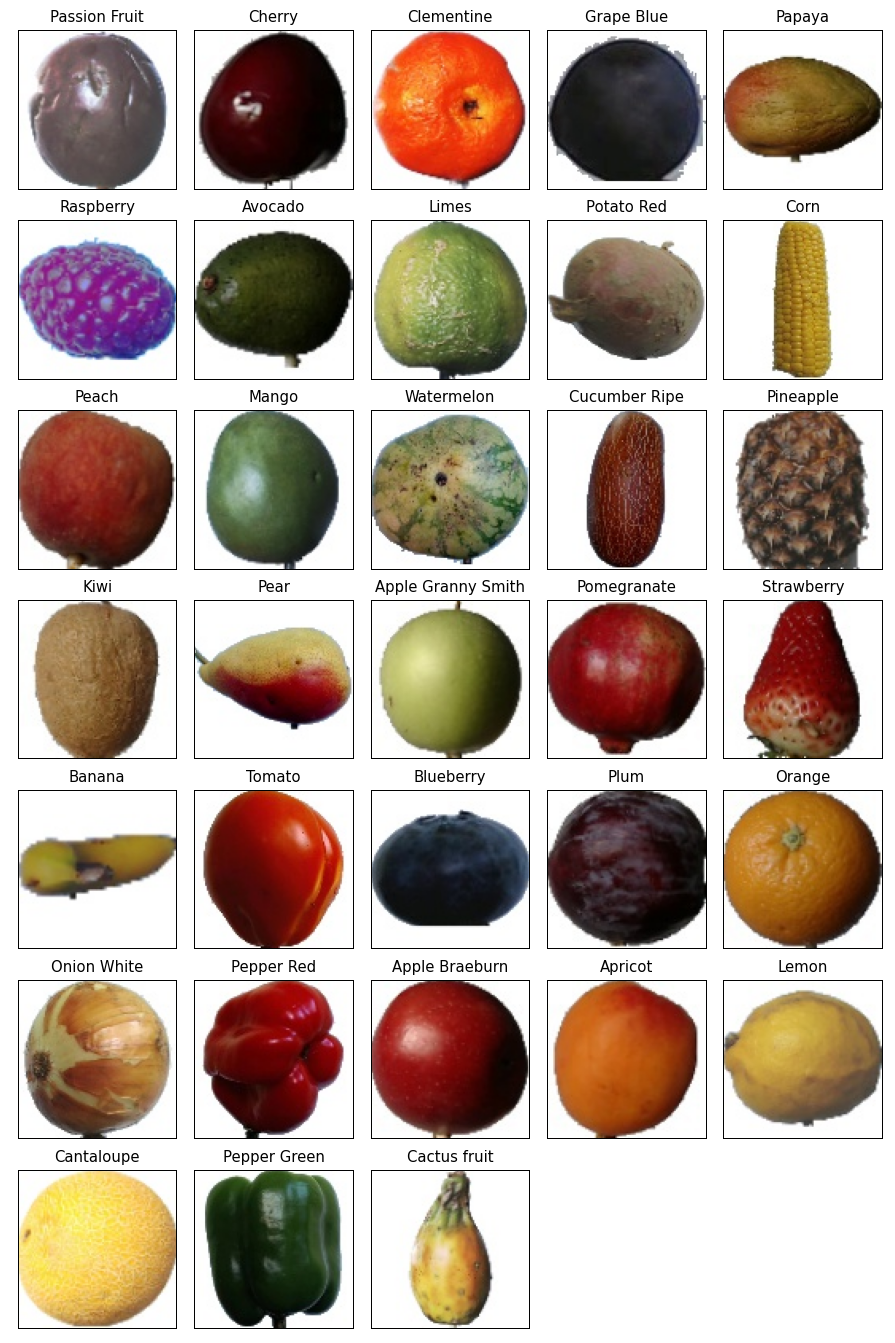
\includegraphics[width=5cm]{training_data.png} }}%
    \qquad
    \centering{{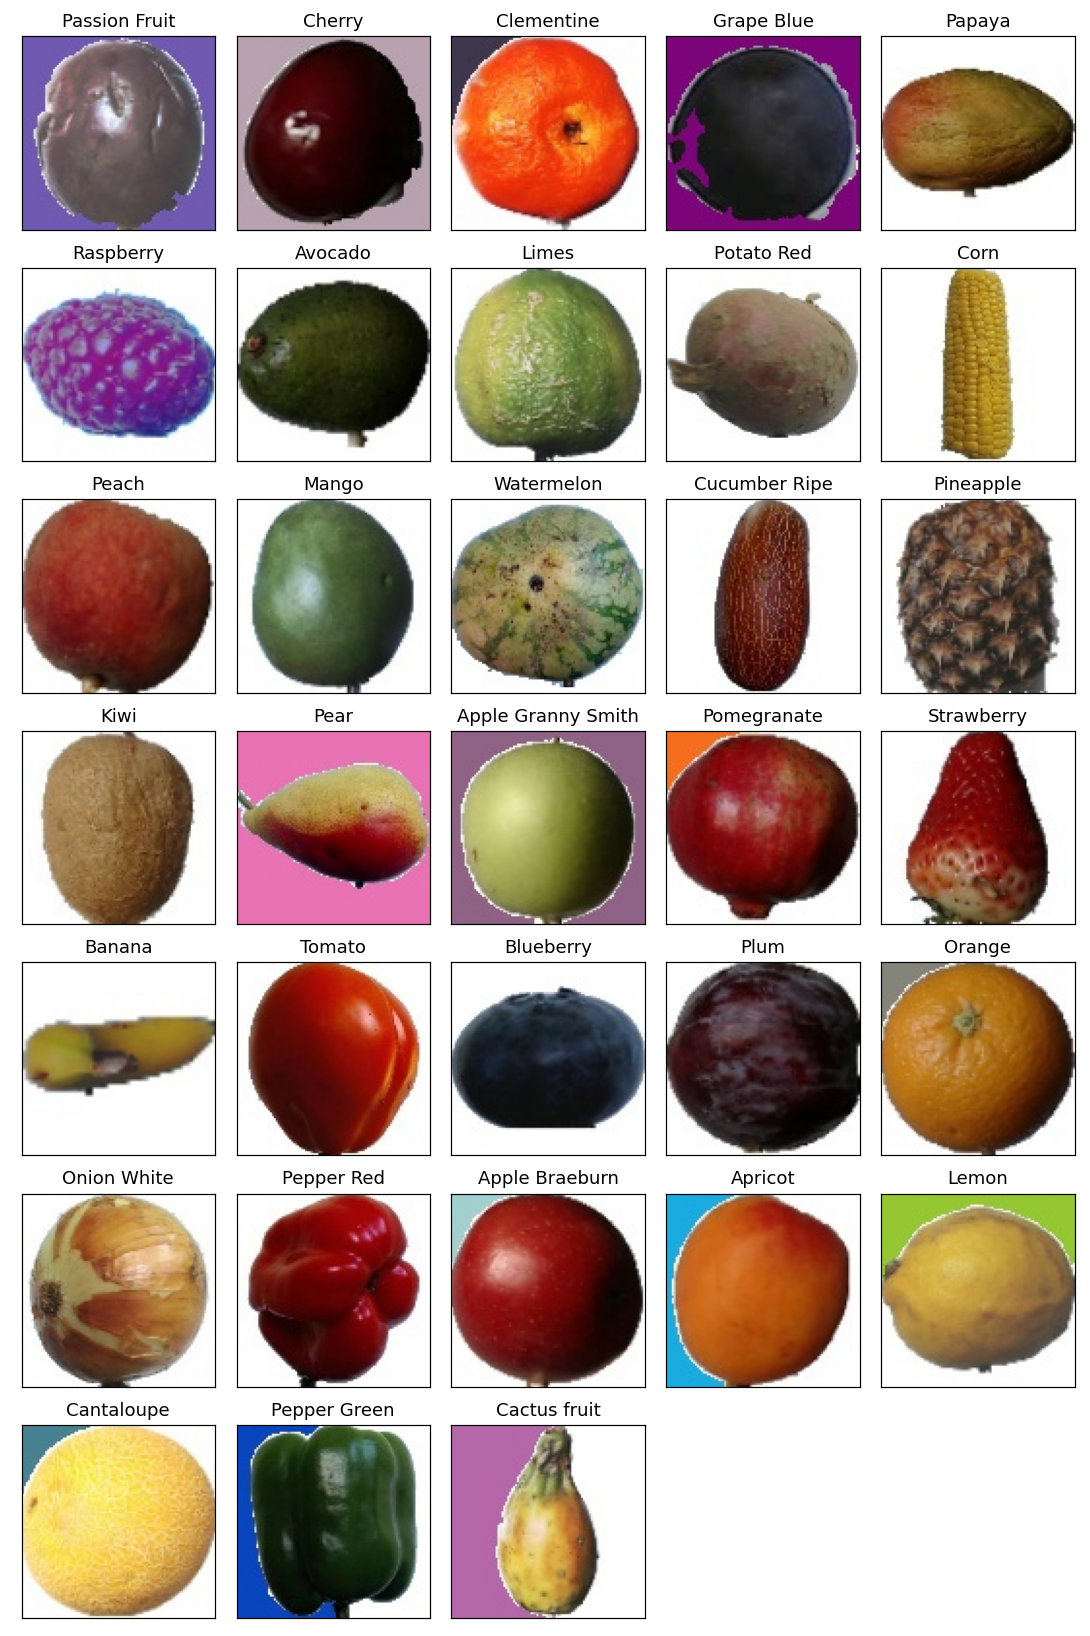
\includegraphics[width=5cm]{train_aug.png} }}%
    \caption{\centering Samples from each fruit class of initial training data (left) and the augmented training data (right)}%
    \label{fig:example}%
\end{figure}

\subsection{Network Architecture and Hyperparameters}
The model utilizes an Adam optimizer with a learning rate of 0.001 and takes in 100x100 pixels images in 3 channels (Red, Green, and Blue). The architecture consists of two identical sets of convolutional and pooling layers that feed into a flatten layer (Figure 2). The flatten layer feeds the one-dimensional data directly into an output layer that uses the softmax activation function to classify the fruit by creating a probability distribution that forces each weight of the output layer to sum to 1.0 \cite{mitchell2024cs63}. Both convolutional layers consist of five filters that are 3x3 pixels in stride and use the rectified linear unit (ReLU) as the activation function, which mitigates the vanishing gradient problem \cite{mitchell2024cs63}. After each convolutional layer, a MaxPooling2D layer with a kernel of size 2x2 was utilized to downsample the 2D spatial data by taking the maximum value over the input window. The output layer has 33 nodes, equal to the number of classes in the Public Fruits Classification Dataset. 

\begin{figure}[h]
\begin{center}
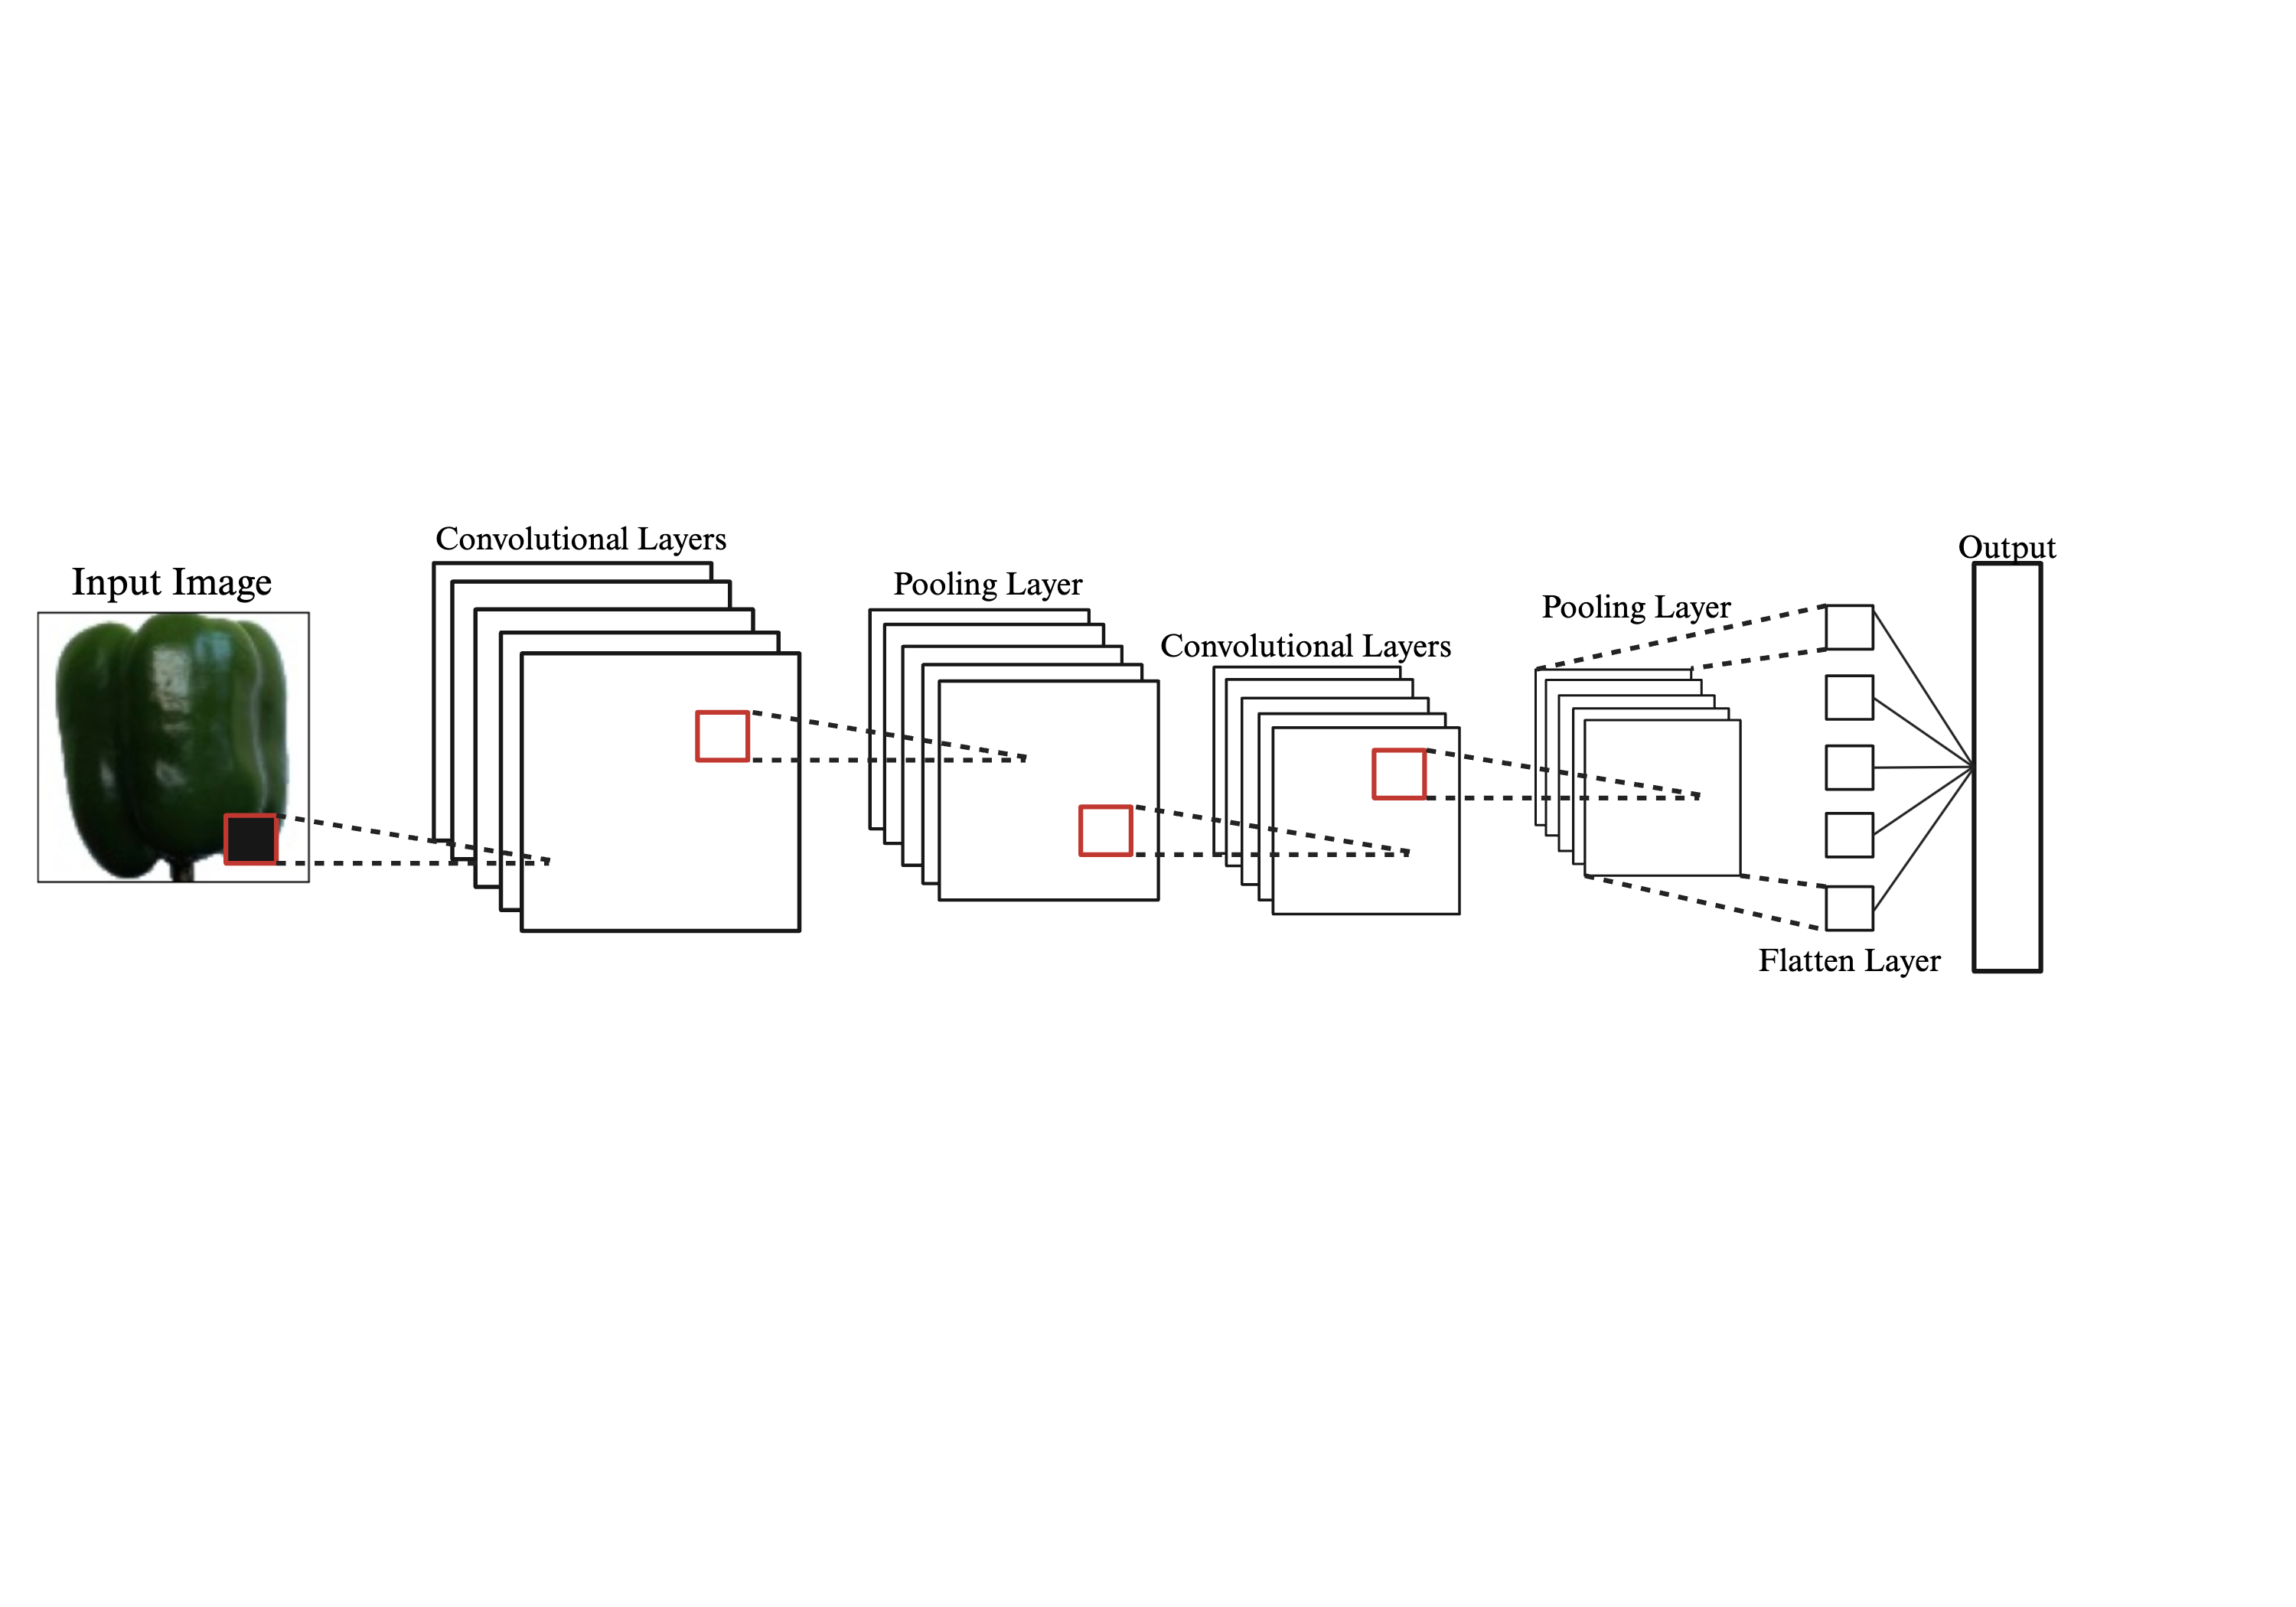
\includegraphics[scale=0.7, trim={0 6cm 0 5cm}, clip]{Project CNN Architecture.png}
\end{center}
\caption{Visual representation of the network architecture without any fully connect layers}
\label{network}
\end{figure}


\subsection{Training Procedures}
Our model is first trained on the initial training data where the fruits and vegetables are centered on a plain white background. The images are propagated through the model and tested against the initial test data. Once high accuracy is achieved, we test our model on the augmented test data with half of the images containing colored backgrounds. Finally, we train our model on the augmented train data and test against the augmented test data. In all three instances, we allowed the model to train for 10 epochs to avoid overfitting as the validation loss began to increase around 12 epochs. 

\section{Results \& Discussion}
When designing our model architecture, we found that the model's accuracy and ability to generalize well for novel examples did not improve with fully connected layers nor did it harm the network's performance when these layers were absent. Although batch normalization for every layer \cite{krizhevsky2012imagenet} and dropout layers can increase the accuracy of the network \cite{krizhevsky2012imagenet}, we found that the model's performance did not drastically improve with these features. Hence, we were able to reduce the number of trainable parameters to 87,688 and thereby decrease computational expense by removing all fully connected layers.

\subsection{Model Accuracy and Generalizability on Novel Test Data}
In our initial evaluation of the network architecture, the CNN is trained and tested on images of fruits with white backgrounds, the model yielded an average of close to 100\% accuracy over the course of 10 trials (Figure 3, Table 1). On rare occasions, the model will incorrectly classify a grape as a blueberry or a banana as corn, but more frequently, none of the fruits or vegetables were categorized incorrectly. The few mistakes indicate that the model likely takes both color and shape of the images into account when classifying the fruit and does so with high performance.

When the model is trained on the initial train data but tested on augmented test data, the accuracy drops to an average of 92.3\% (Table 1, Figure 4) over the course of 10 trials. In almost all of the trials, all of the misclassified images had either partially or fully colored backgrounds, indicating that the model likely analyzes the background of the image to a certain degree and feeding the model an input with a colored background has a higher potential for misclassification. The most commonly misclassified fruits include bananas, pears, and red potatoes and the most common wrong answers were ripe cucumbers followed by green peppers, cactus fruits, and cantaloupes. Because ripe cucumbers in the dataset display a wide range of colors, ranging to brownish red to green, and have various shapes (especially when viewed from a variety of orientations) they are the most common wrong answers produced by the model. Yet, the CNN's high accuracy of correctly classifying the majority of images with colored backgrounds, not in the training data, demonstrates the model's strong ability to generalize its learning to novel examples. 

To further evaluate the model's accuracy and generalizability, we compared the performance of the model trained on the initial data but tested on the augmented data to the model's performance when trained on the augmented train data and tested against the augmented test data. When trained on the augmented data, the model's average accuracy across 10 trial runs was 99.88\% (Table 1, Figure 5), indicating that the model is able to learn to ignore colored backgrounds to a large degree and correctly classify the fruits. When evaluating the few errors made in each trial run, 65.4\% of the images had colored backgrounds, indicating that the model performs slightly better on classifying fruits on a blank white background compared to the fruits with colored backgrounds.

Despite the model's strong performance in all three cases, the results should be interpreted with discretion. Since the fruits are all centered in the image, the model may have possibly learned to increase the weights on the nodes corresponding to the center of the image. In addition, the method implemented to change the background left a slight white gap between the colored background and the fruit, potentially leading the model to analyze the white gap to determine the shape of the fruit. Compared to other common image classification sets such as the mnist \cite{mnist_tensorflow} and the fashion-mnist \cite{fashion_mnist_tensorflow} datasets, the images of the fruits are higher in resolution. Furthermore, the backgrounds of the images within both the real and test data were not realistic and the model would likely perform more poorly on more realistic images of fruits with various backgrounds and images containing multiple of the same fruit. Hence, our model may not generalize well to other images of fruits that deviate from the format in the TJ NMLO Public Dataset Fruit Classification.

\begin{figure}[t]
\begin{center}
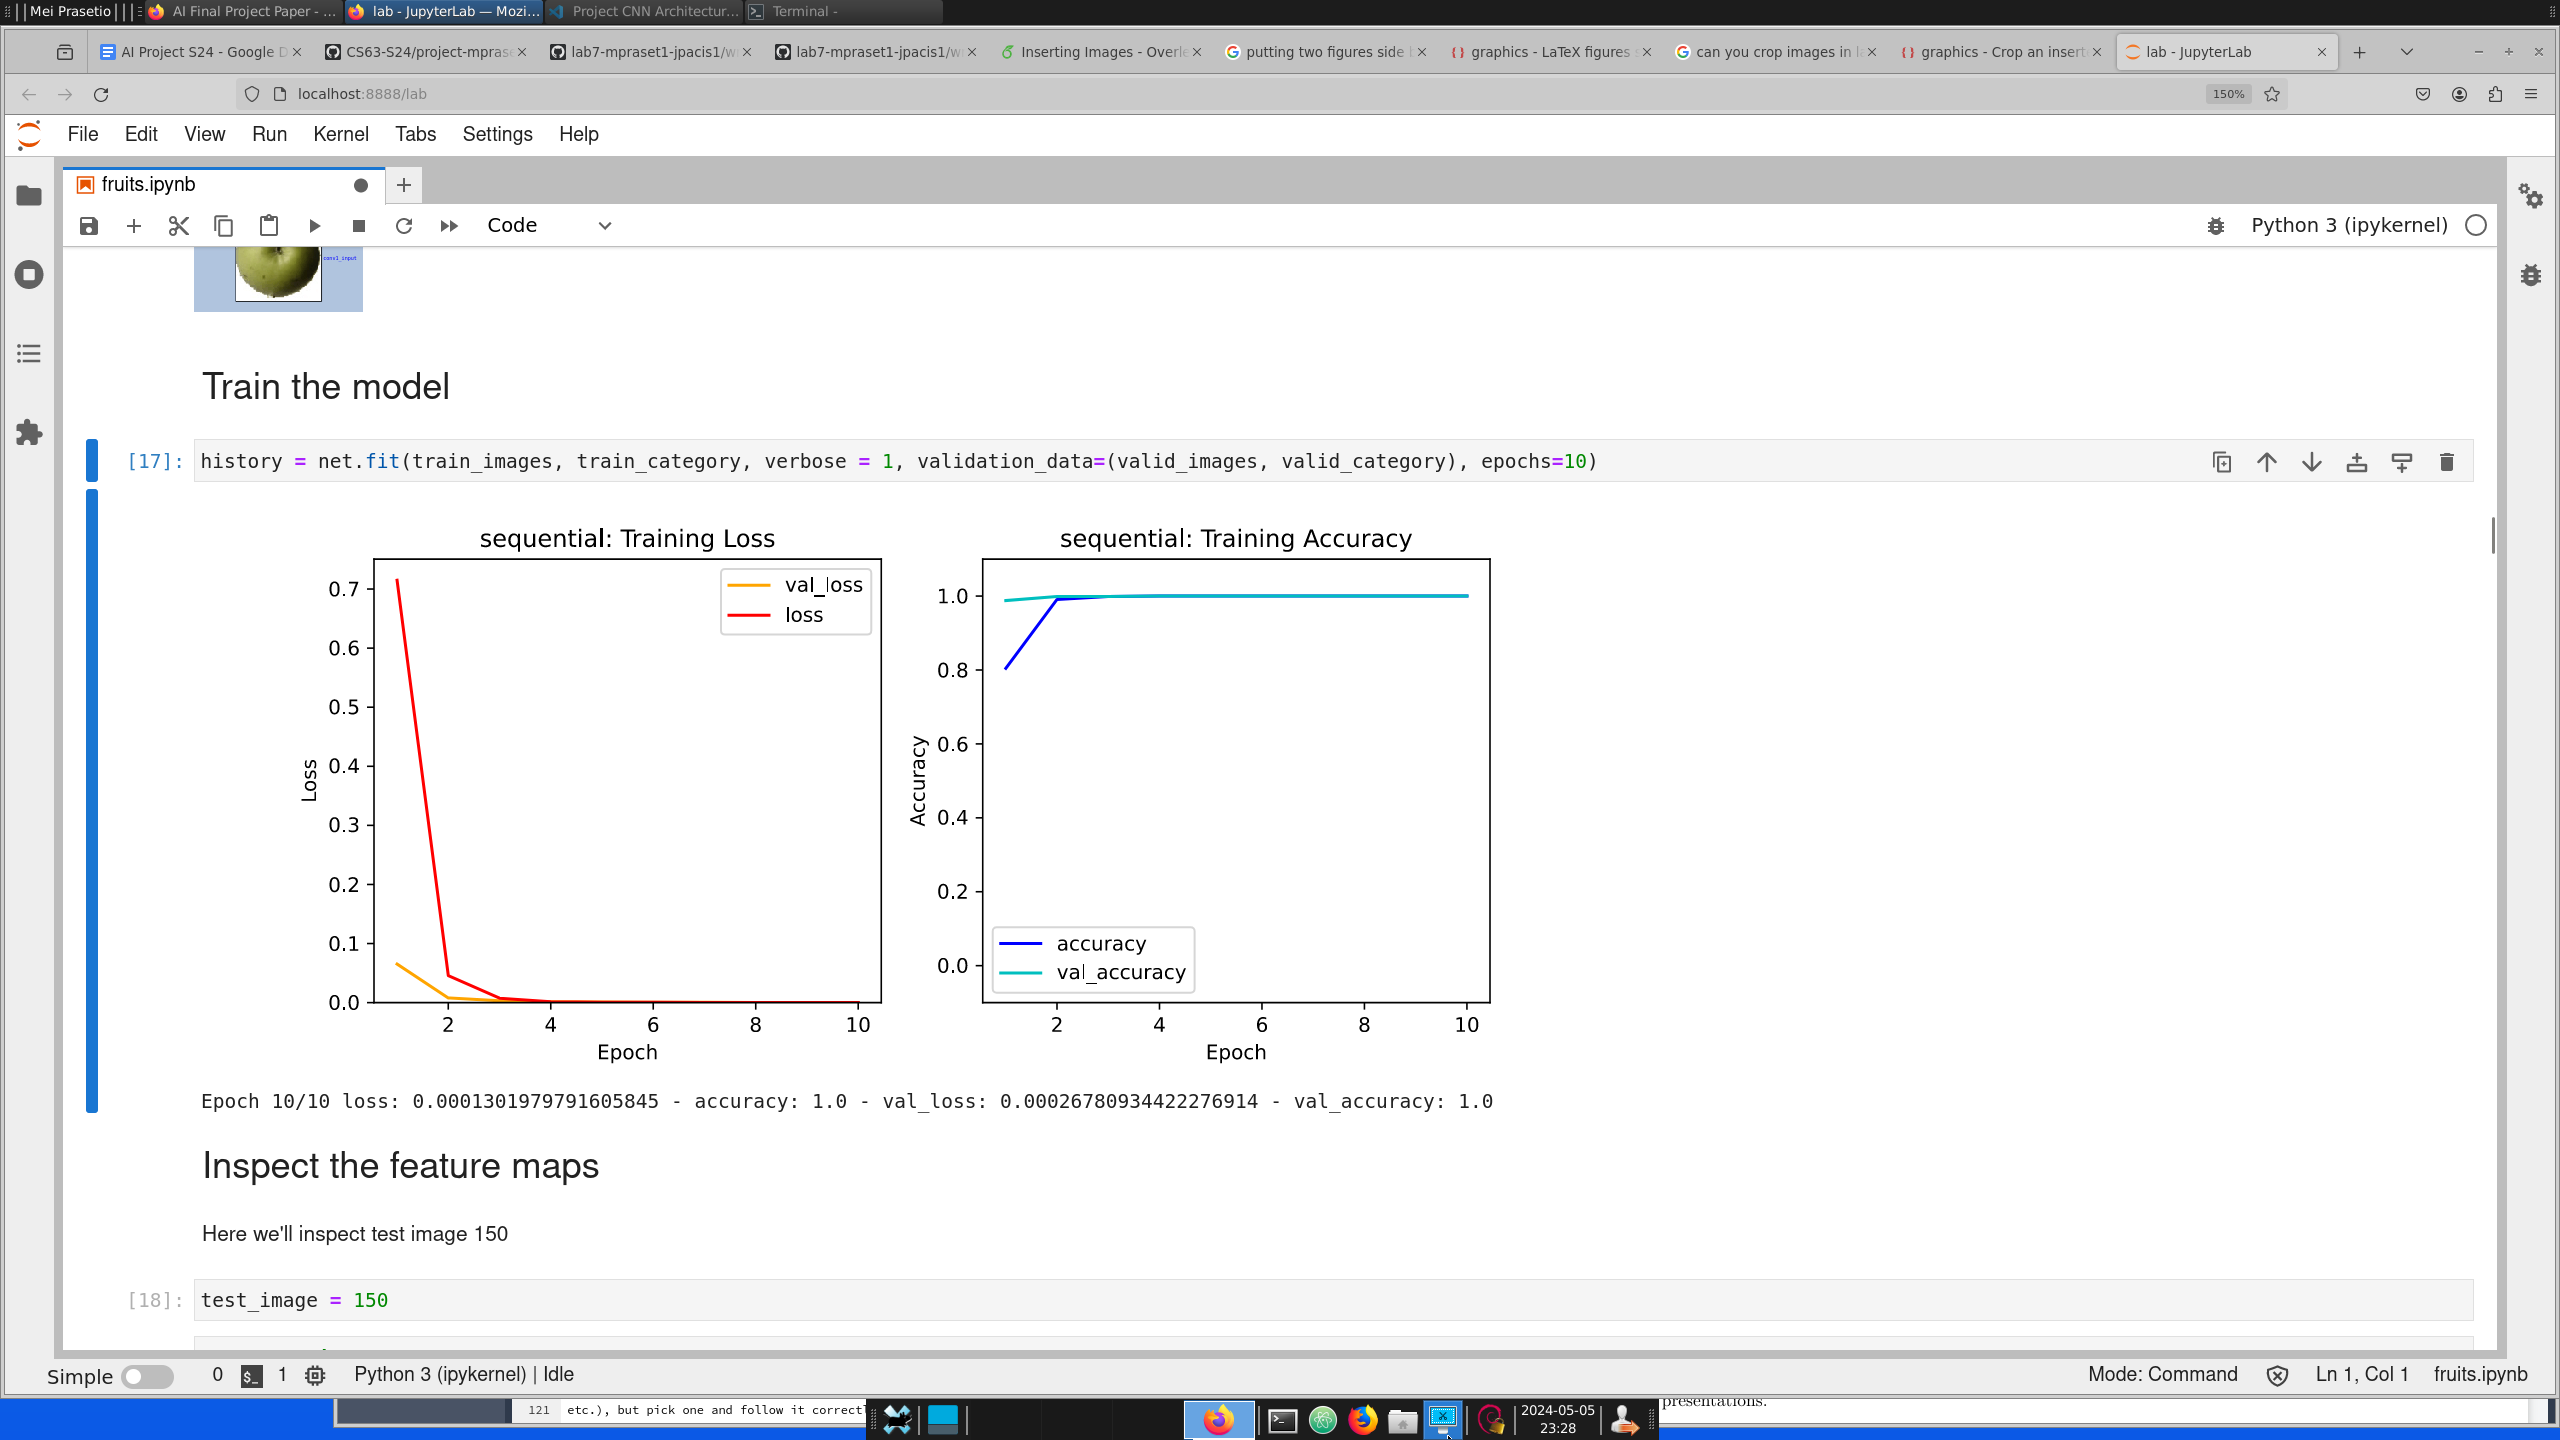
\includegraphics[scale=0.3, trim={5cm 10.8cm 18cm 17cm}, clip]{train_model.png}
\end{center}
\caption{\centering Representative sample of a loss (left) and accuracy (right) throughout training on initial data.}
\label{Train Model}
\end{figure}


\begin{table}[htbp]
\centering
\begin{tabular}{||c|c|c|c||} 
 \hline
 Train Data & Test Data & Average Accuracy & Average \# Errors\\ [0.5ex] 
 \hline\hline
 Initial & Initial & 0.9999 & 0.4\\ 
 \hline
 Initial & Augmented & 0.9233 & 342.96\\
 \hline
 Augmented & Augmented & 0.9988 & 5.2\\
 \hline
\end{tabular}
\caption{\centering Average accuracy on test data and the average number of errors made by the model given different sets of train and test data.}
\label{tab:accuracy_errors}
\end{table}


\begin{figure}[p]
\begin{center}
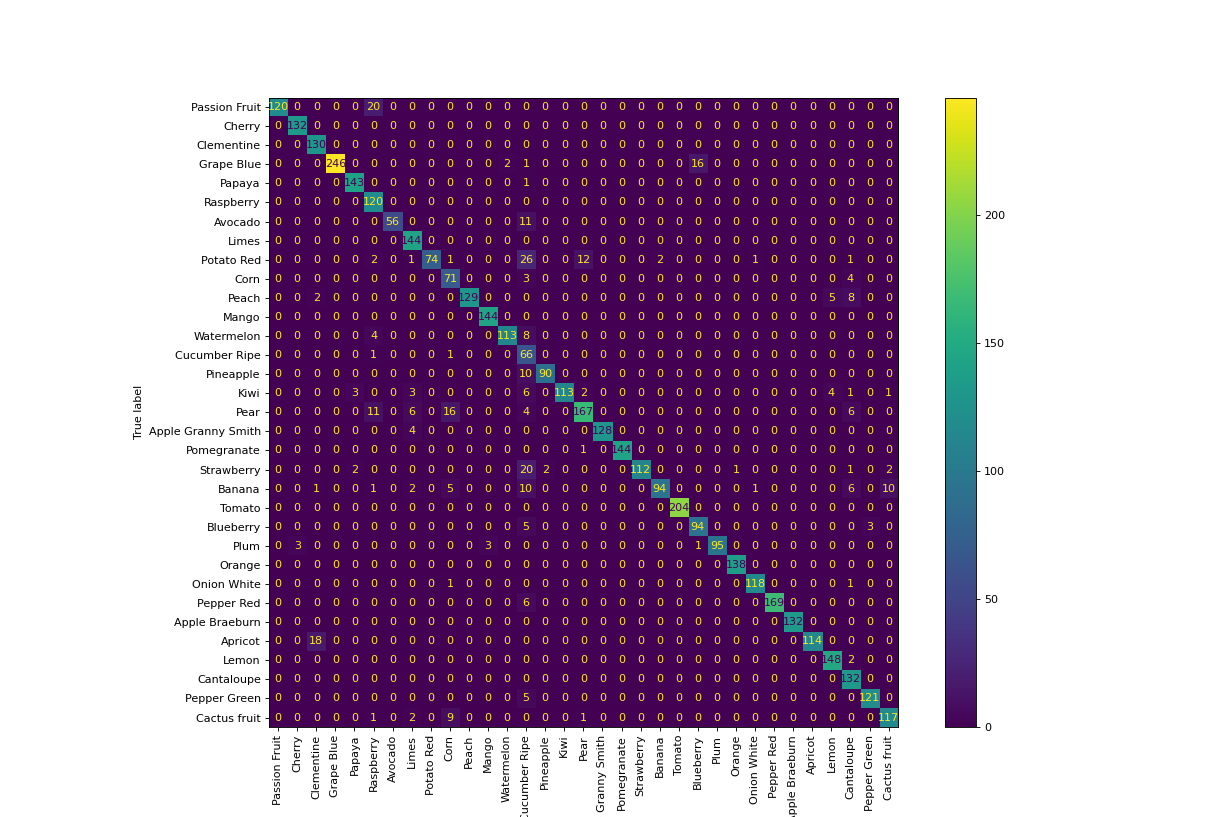
\includegraphics[scale=0.28]{conf_matr_2.png}
\end{center}
\caption{\centering A sample confusion matrix of the CNN's mistakes in classifying augmented images of fruits from training on the initial data.}
\label{Confusion Matrix}
\end{figure}
\begin{figure}[p]
\begin{center}
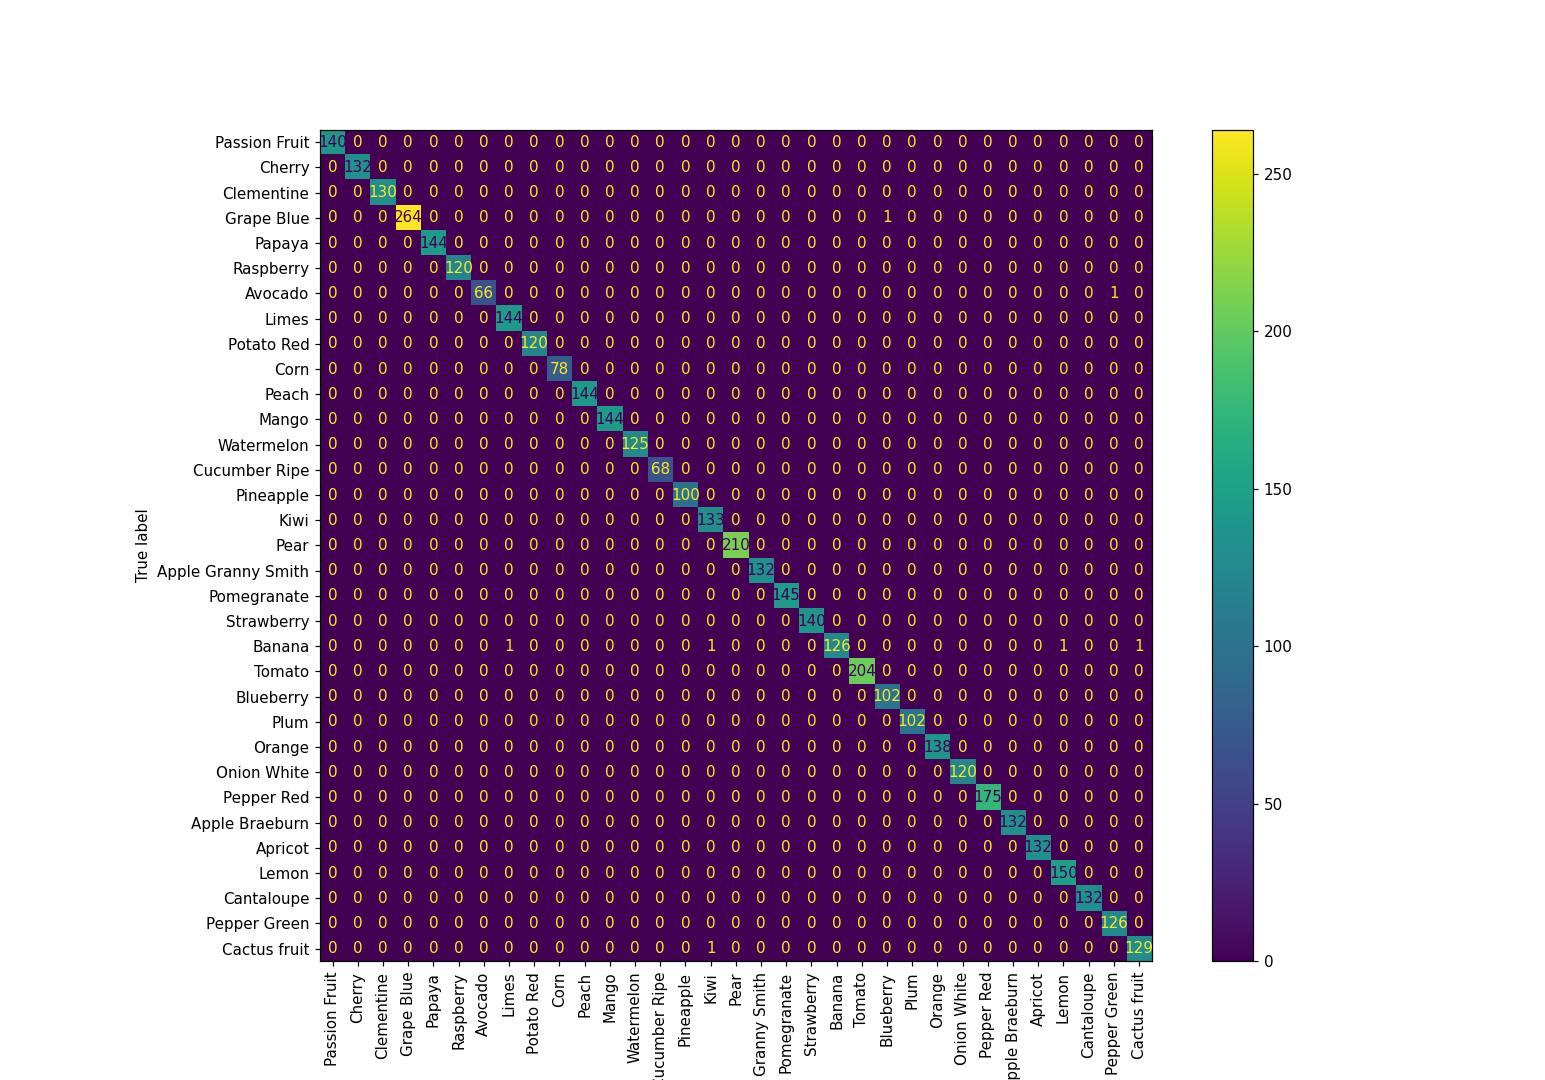
\includegraphics[scale=0.21]{conf_matr_3.png}
\end{center}
\caption{\centering A sample confusion matrix of the CNN's mistakes in classifying augmented images of fruits from training on the augmented data.}
\label{Confusion Matrix2}
\end{figure}
\clearpage

\section{Conclusions}
In an attempt to create a computationally inexpensive model that is able to generalize well on novel tests, we trained our CNN that lacks fully connected layers on the TJ NMLO Public Fruits Classification Dataset. We found that a model architecture consisting of solely convolutional and pooling layers is able to classify images of fruits on a plain white background with very high accuracy despite lacking fully connected layers that feed into the output layer. Furthermore, we found that when the model was trained on the initial test data, it is able to generalize well on augmented test data containing the images of fruits with colored backgrounds. While the performance of the model does noticeably increase when trained on the augmented test data, the model shows promise in generalizing its training on initial data to relatively simple image augmentations. 

Further work is needed to determine the model's generalizability to more realistic data. By testing the model against fruit images with multiple colors and patterns in the backgrounds, the architecture can be adjusted accordingly. With more complex images where there are multiple fruits, the fruits are not centered, or the background is a kitchen, supermarket, orchard, or another context with multiple background objects, the model may need to eventually utilize fully connected layers to correctly classify the fruits. But for images that are uniformly formatted and contain one object, we demonstrate that a CNN consisting of only convolutional and pooling layers displays high accuracy and generalizability to novel examples. 

\section{Acknowledgements}
We would like to thank Professor Lisa Meeden for her input during the brainstorming portion of our project, helping us pick a suitable data set for our project, and providing written feedback on our project checkpoint. We would also like to thank both Professor Lisa Meeden and Professor Ben Mitchell for their help in both the data preprocessing phase and utilizing aitk to visualize our CNN. 
In addition, we found many of the libraries used for preprocessing the dataset from Kaggle user Johannes Hedström's public Dataset Notebook from this competition \cite{100_accuracy_fruitdataset}. Our method of augmenting the data was inspired by Stack Overflow user Rotem's answer to the public forum titled ``How can I change background color to red of an image using Python" \cite{stackoverflow_redbackground}. Finally, we would like to thank the students in Lab B of CS63 Spring 2024 for their feedback on our projects during the checkpoint presentations. 
\clearpage

\bibliography{yourbibfile} 
\bibliographystyle{ieeetr} 


\end{document}

